\chapter{Introduction}\label{chp:intro}
%\vspace{-1.5cm}
%\noindent\rule{\columnwidth}{1.2mm}
%\vspace{0.1cm}

The robot development in the last century was able to revolutionize the industry by providing flexibility, reliability and quality to the production line, since robots often can perform tasks faster, more accurately and with fewer errors than humans. Human labor that was often repetitive and risky was steadily replaced by robotic labor, with precise movements and increasing automation over time, as shown on \prettyref{fig:robots-per-workers}.

\begin{figure}[!ht]
    \centering
    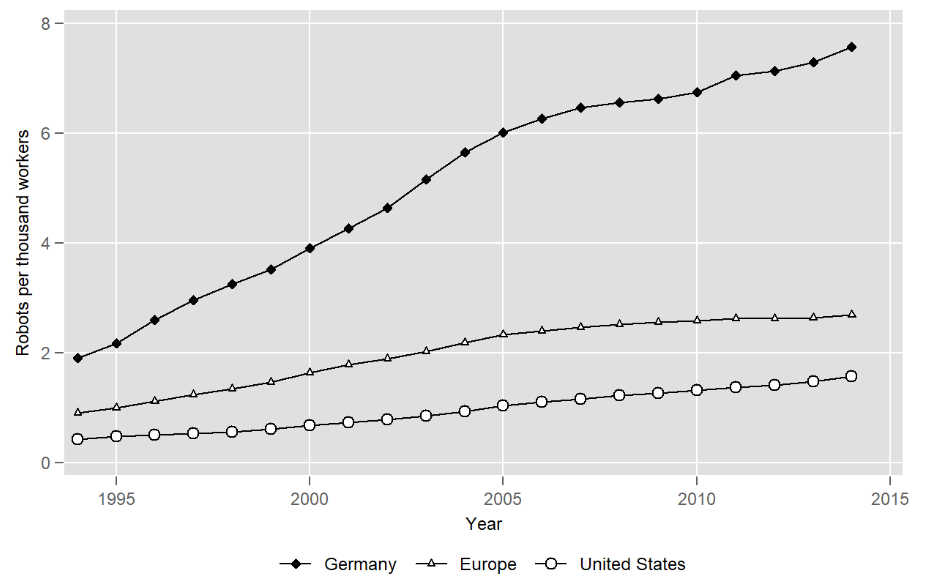
\includegraphics[width=.8\linewidth]{robots-per-workers}
    \caption{Robots per thousand workers in the industry from 1995 to 2014 \cite{dauth2017german}.}
    \label{fig:robots-per-workers}
\end{figure}

Even though robots are increasingly present in the industry, using robots to assist persons in everyday life might be more challenging. Many authors propose their use in places like schools, hospitals, and homes, including wheelchair robots, companion robots, manipulator arms for the psychically disabled and elderly populations, etc \cite{feil2005defining}. However, the dynamic and heterogeneous environment, the energy constraints and the safety are still issues in domestic use robotics.

According to Feil \cite{feil2005defining}, assistive robots are defined as ones that give support to a human user, whereas socially interactive robots are the ones that merely can interact with humans in the form of gestures, speech, etc. The intersection between these two groups is called socially assistive robots, not focusing on the interaction itself but using it as a mechanism to provide aid or assistance.

Fong \cite{fong2003survey} defines 8 traits in socially interactive robots:

\begin{itemize}
    \item Embodiment: defined as the body capabilities of the robot, the morphology, and design to deal with the ambient. Social robots design is often taken into consideration because the user must be comfortable engaging with the robot. Also, the number of sensors and actuators the robot has will expand its capabilities.
    \item Emotion: complements the embodiment in the robots by interacting in a social context. Integrating emotion in robots can create empathy and make people treat them like they treat other humans. Emotions can be displayed both as an expression, in the form of moving lips, eyebrows, eyes, and LEDs, as well as in the form of speech, in voice tone, loudness, and pitch. Body language also takes place in full-body robots.
    \item Dialogue: Creating a meaningful dialogue between two or more parties is hard even in the form of low-level dialogue. Natural language processing are still features under development and remain a great challenge to robots. Robots can also use dialog in a non-verbal way, communicating in gestures and facial display, in addition to displaying emotions.
    \item Personality: in order to correlate with users, robots must develop personality traits that will distinguish them from other robots.
    \item Human-oriented perception: to interact, robots must perceive the environment as humans do. In social situations, this includes people tracking, speech recognition, gesture recognition, and facial perception.
    \item User modeling: in addition to design and perception, they must act based on people personality, learning the user's personality to create a model on how to react.
    \item Socially situated learning: continuously learning for improving communication or acquiring new skills is essential, whether by teaching or imitation.
    \item Intentionality: lastly, humans must feel that the robot has a purpose and acts rationally. This can be achieved by demonstrating goal-directed behaviors or demonstrating attention to key objects in the scenario.
\end{itemize}

Feil goes further and defines the socially assistive robot with additional properties relative to Fong's definition:

\begin{itemize}
    \item User Populations: defines the characteristics of the user, like age, impairment, and need. He categorizes the user populations as elderly, individuals with physical impairments, individuals in convalescent care, individuals with cognitive disorders and students.
    \item Task: the author cites as task examples tutoring, physical therapy, daily life assistance, and emotional expression.
    \item Sophistication of interaction: the robot must develop beyond the emotional feature described by Fong, evolving into more complex reciprocal interactions with the user.
    \item Role of the assistive robot: the role of the assistive robot must reflect into its appearance and behavior, affecting both embodiment and personality, depending on the task and nature of the interaction.
\end{itemize}

\begin{figure}[!ht]
    \centering
    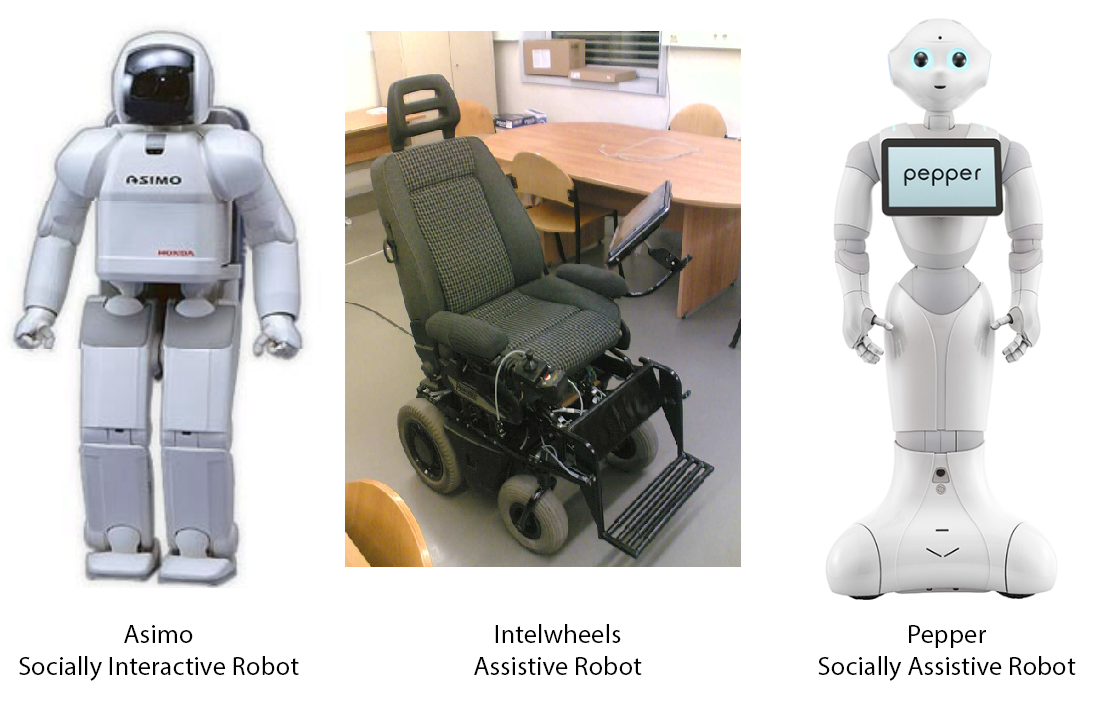
\includegraphics[width=\linewidth]{social-assistive-robots}
    \caption{Examples of Assistive and Social robots \cite{sakagami2002intelligent,braga2008intellwheels,tanaka2015pepper}.}
    \label{fig:social-assistive-robots}
\end{figure}

One of the most famous socially interactive robots developed is ASIMO, shown on the left on \prettyref{fig:social-assistive-robots}, a human-like robot developed by the Japanese company Honda in 2000. It featured a pair of legs and many features and sensors that would later be integrated into other assistive robots. Its main task was to meet visitors in the meeting room and to guide them once the manager confirms their identity. It was able to perform navigation, obstacle avoidance and respond to voice and gesture calls \cite{sakagami2002intelligent}. Even though the robot can interact with people, it does not qualify as a socially assistive robot (the first version, at the time) as defined by Feil because it couldn't fit in the user populations described. The robot was later improved to have greater grasping capabilities and a more robust sensor set.

Intelwheels is an example of an assistive robot, as seen in the middle of \prettyref{fig:social-assistive-robots}. It can assist handicapped people operating an electric wheelchair, providing not only user operation with collision avoidance but autonomous navigation. It can help elders and people with physical impairments, but the user input is one-way: it can recognize voice and facial expressions but won't interact back with the user \cite{braga2008intellwheels}.

Pepper, seen on the right on \prettyref{fig:social-assistive-robots}, was developed to fit into the category of both emotional expression and tutoring. It was aimed at the concept of the robot learning together with children using the robot's display to teach English, characterizing it as a socially assistive robot. A remote human teacher would help the process by orienting the classes. Instead of just showing the contents in the screen, creating boredom, the robot engaged in playful activities with the kids, including telling them to search for a specific object in the room or repeating gestures with the robot, compelling the children to participate actively \cite{tanaka2015pepper}.

The Care-o-bot, or COB, for short, is described as a robotic home assistant aimed at helping people with mobility impairments in their daily lives. The target group includes elders, disabled, people with health conditions and with movement restraints. Its tasks include setting the table, carrying objects like books and drinks around, dealing with medication, helping the patients standing up, as well as serving as a companion to the person. The robot can also do other tasks usually performed by a nurses and doctors, like monitoring the patient with conditions in their daily routines, reminding them to take medication and calling emergency in case of incidents \cite{graf2004care}.

\begin{figure}[!ht]
    \centering
    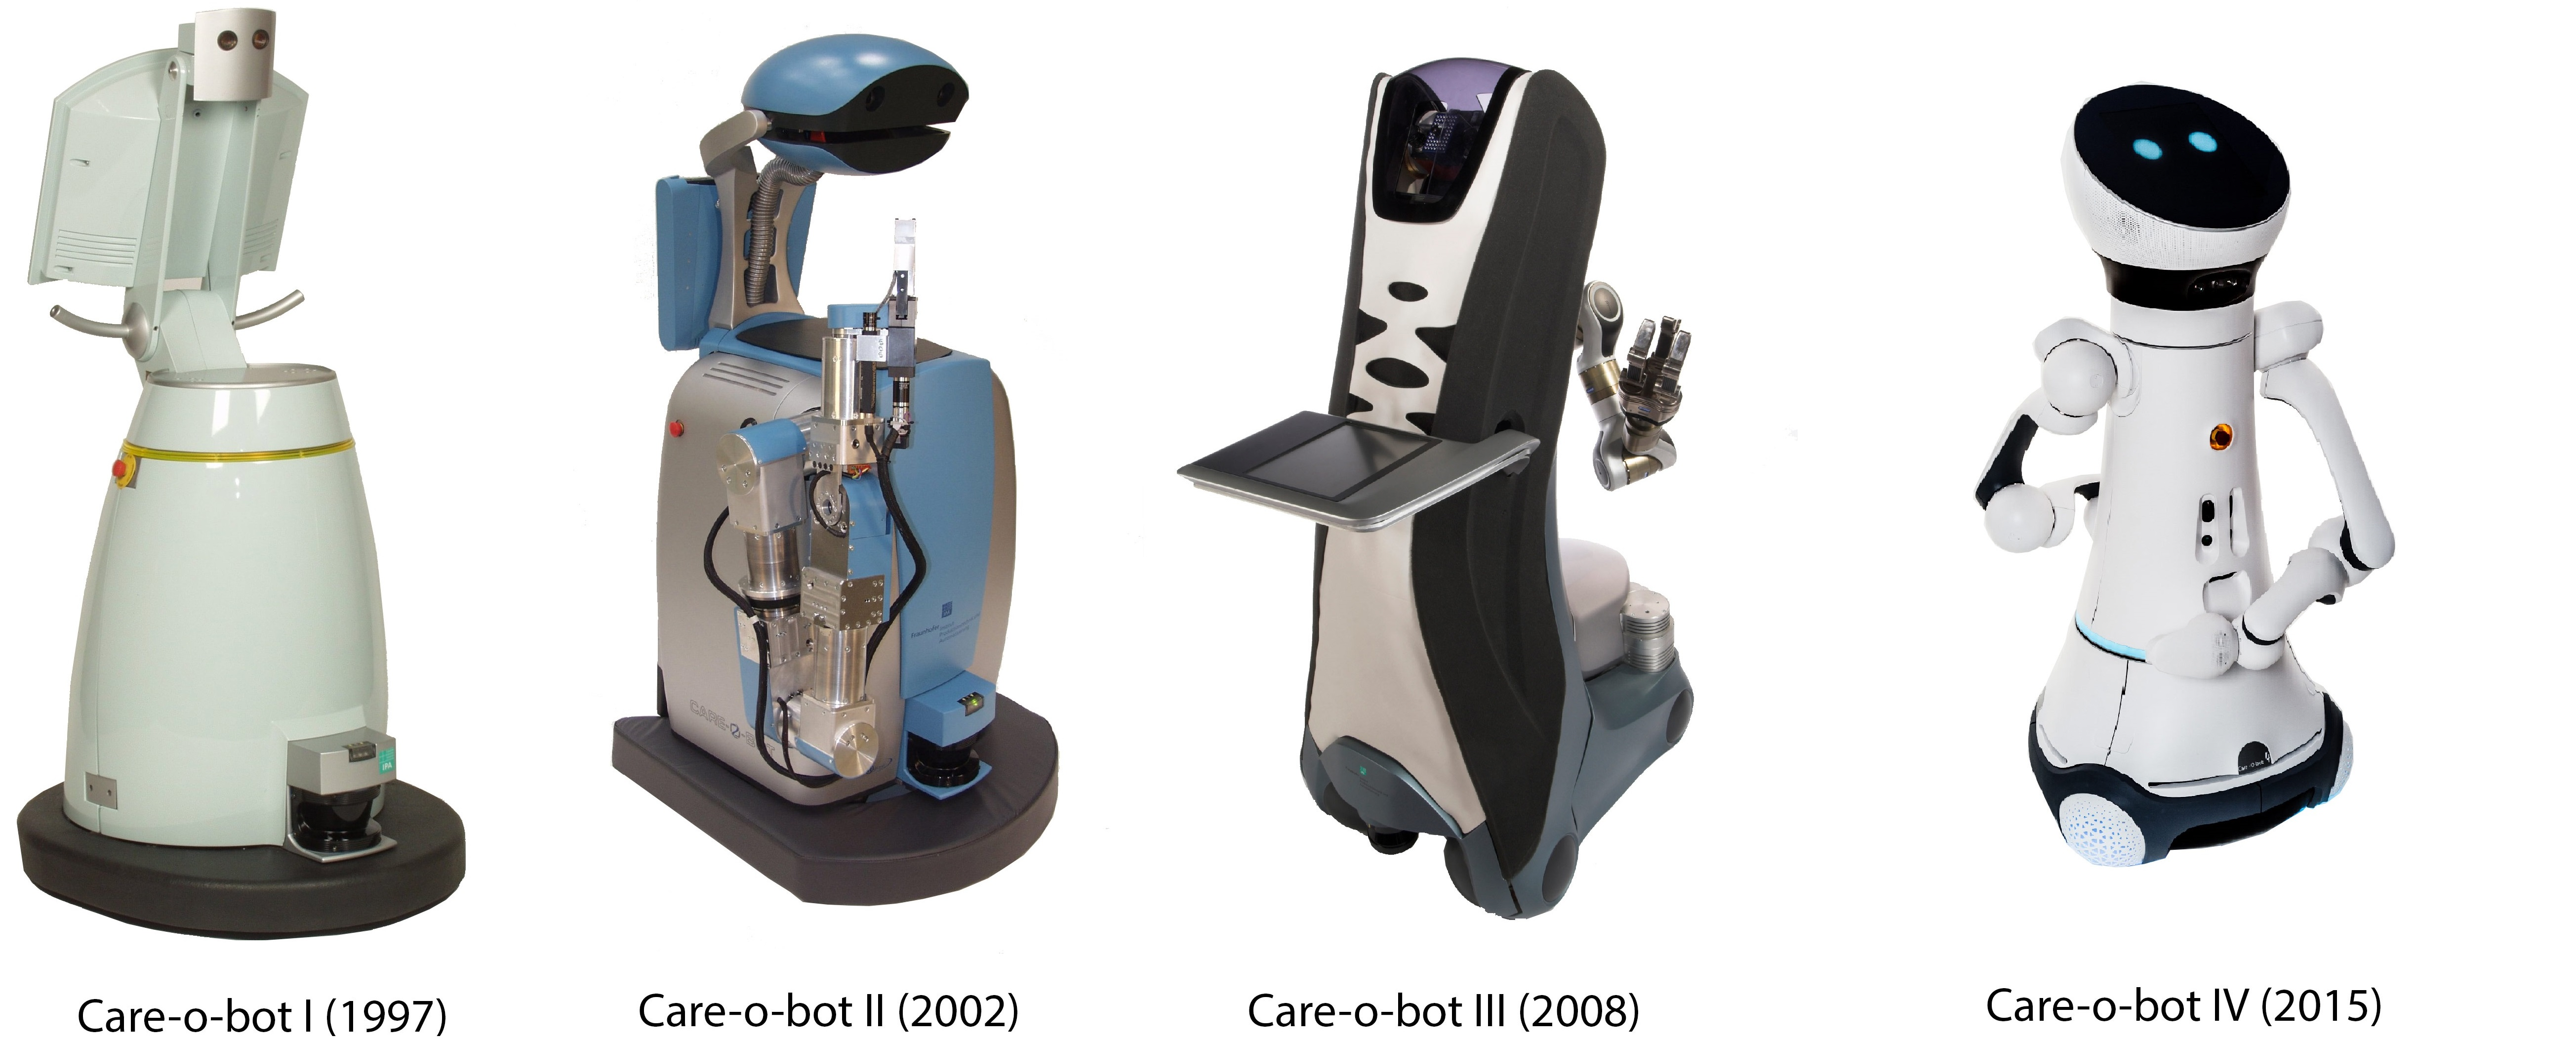
\includegraphics[width=\linewidth]{cob-evo}
    \caption{Evolution of Care-o-bot.}
    \label{fig:cob-evo}
\end{figure}

The Care-o-bot evolution throughout the years can be seen on \prettyref{fig:cob-evo}. The first prototype was built in 1997, but it didn't pack many capabilities as the technology was very limited. It was soon followed by Care-o-bot II, in 2002, equipped with a manipulator, two cameras, laser scanners, and a hand-held control panel. Version II presented great improvements in navigation, computer vision, and manipulation, but was still rudimentary, having problems in low light conditions and dynamic environments (the 3D scans could only be run once because of processing constraints) and was not recommended for inexperienced users \cite{graf2004care}.

The third generation came in 2008, using a better 7DOF arm and 3 finger gripper with tactile feedback. It also became a lot more user-friendly, applying the concepts of embodiment and presenting a less bulky body with smoother surfaces and less visible mechanical parts. The robot body was divided into a working side (in the back, where the manipulator stands) and a serving side (on the front, to interact with users) \cite{graf2009robotic}.

The fourth generation was presented in 2015 and focused heavily on emotion design. It was developed to appear familiar and sociable, and avoid the uncanny valley \cite{mori2012uncanny}, where human-like robots can cause strangeness or even fear. It featured a multi-modal user interface capable of displaying facial expressions with a minimalistic pair of eyes to display a wide range of emotions. The spherical joints in the torso and head allow more agility, the body is smaller and more efficient and more sensors and 3D cameras were installed.

One of the many challenges of assistive robots is navigating the environment. As they need to reach places in the house like the kitchen or the bedroom, they sometimes need to be aware of how to navigate through the rooms and corridors to reach the final destination. The approach described in \citeauthor{siegwart2011introduction} for this problem is running algorithms in different layers: perception, to extract meaningful data from the environment using available sensors; localization, to determine where it is relative to the environment; cognition, in order to take action given the inputs; and motion control, in order to output the right commands to the motors \cite{siegwart2011introduction}. \prettyref{fig:navigation_guidelines} shows us the guidelines to build a localization stack in a mobile robot.

\begin{figure}[!ht]
    \centering
    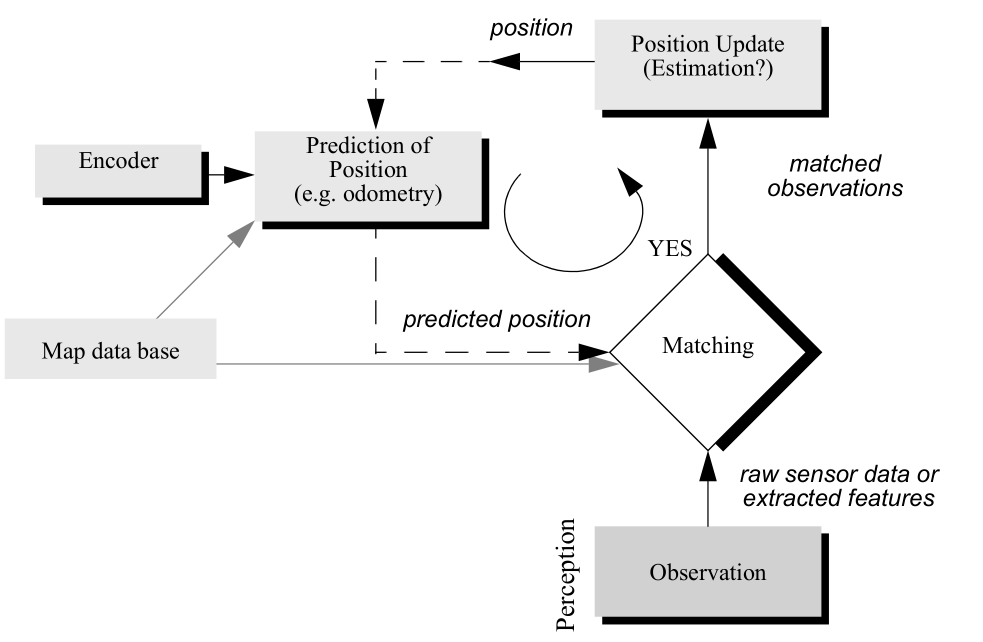
\includegraphics[width=0.8\linewidth]{navigation_guidelines}
    \caption{Localization stack flowchart \cite{siegwart2011introduction}.}
    \label{fig:navigation_guidelines}
\end{figure}

As we can see, it is necessary to sense the state of the robot and the world. This is done through encoders in the wheels, GPS, or other forms of localization, in the form of odometry, or in observations, using 3D cameras, LIDAR, Sonar, etc. This data is fed to a matching algorithm, together with a map database, resulting in an estimated position update, that will be used as feedback for the next iteration.

However, this approach is only as accurate as the map is. Many algorithms aim to solve the mapping problem accurately, but there is no standard way of telling how accurate each algorithm is because there is no agreement on which benchmarks to use. The difficulties in comparing visual data and the absence of the ground truth impose challenges when comparing maps generated by different algorithms \cite{amigoni2007good}.

\section{Objectives}

The goal of this paper is to propose a method for comparing mapping algorithms. We will test the proposed architecture against the most popular algorithms available in the open repositories, namely Gmapping, Hector, Karto and Cartographer, using data from simulated Care-o-bot. The results will be then discussed and compared against what is currently present in the literature about mapping benchmarking. 

The following tasks are specific objectives:

\begin{itemize}
    \item Revision of literature for SLAM comparison metrics.
    \item Implement an algorithm for the generation of maps based on the ground-truth representation.
    \item Simulation of proposed SLAM algorithms in the Care-o-bot robot.
    \item Comparison of results using proposed metrics.
    \item Publish all test data and algorithms in an open-source repository.
\end{itemize}

% revisão
% comparação de mapas

\section{Structure}

This work is structured as follows. \prettyref{chp:fundament} shows the background theory in order to understand how the tests were performed. It includes an introduction to the Robot Operating System (ROS) used in all experiments, as well as an introduction to COB hardware. \prettyref{chp:slam_mapping} explains the mapping problem into more detail and gives an introduction to how each tested algorithm works. This chapter also presents a review of the literature to come up with good metrics and an algorithm approach for comparison. A custom way of generating accurate maps is proposed and simulated using Care-o-bot. The resulting are exported into public datasets, so that they can be reused for further testing or even for different algorithms not tested in this dissertation.

\prettyref{chp:results} shows the results obtained using the proposed metrics and a discussion. Finally, \prettyref{chp:conclusoes} presents conclusions and discusses future work in this topic.

%state the general topic and give some background

%provide a review of the literature related to the topic

%define the terms and scope of the topic

%outline the current situation

%evaluate the current situation (advantages/ disadvantages) and identify the gap

%identify the importance of the proposed research

%state the research problem/ questions

%state the research aims and/or research objectives

%state the hypotheses

%outline the order of information in the thesis

%outline the methodology